% !TEX TS-program = pdflatex
\documentclass[11pt]{article}

% -------------------- Packages --------------------
\usepackage[a4paper,margin=1in]{geometry}
\usepackage{amsmath,amssymb}
\usepackage[T1]{fontenc}
\usepackage{lmodern}
\usepackage{xcolor}
\usepackage{tcolorbox}
\tcbuselibrary{skins,breakable}
\usepackage{enumitem}
\usepackage{hyperref}
\usepackage{tikz}
\usetikzlibrary{calc,angles,quotes,arrows.meta}

\pagestyle{empty}

% -------------------- Dark Theme Colors --------------------
\definecolor{bg}{HTML}{000000}
\definecolor{pairbg}{HTML}{121212}
\definecolor{solbg}{HTML}{0A0A0A}
\definecolor{border}{HTML}{2A2A2A}
\definecolor{text}{HTML}{FFFFFF}
\definecolor{muted}{HTML}{C9CDD3}
\definecolor{gold}{HTML}{FFD700}
\definecolor{green}{HTML}{4ADE80}
\definecolor{cyan}{HTML}{38BDF8}

\pagecolor{bg}
\color{text}

\hypersetup{
  colorlinks=true,
  linkcolor=cyan,
  urlcolor=cyan
}

\setlength{\parindent}{0pt}
\setlength{\parskip}{10pt}

% Help LaTeX avoid overfull lines globally
\sloppy
\setlength{\emergencystretch}{3em}

\setlist[itemize]{left=1.4em,itemsep=6pt,topsep=6pt}
\setlist[enumerate]{left=1.6em,itemsep=4pt,topsep=4pt}

% -------------------- tcolorbox Base --------------------
\tcbset{
  enhanced,
  breakable,
  arc=12pt,
  boxrule=0.8pt,
  left=14pt,right=14pt,top=12pt,bottom=12pt
}

\newtcolorbox{QAPair}[1]{%
  colback=pairbg,
  colbacklower=solbg,
  colframe=border,
  coltext=text,
  title=\textcolor{gold}{\bfseries #1},
  fonttitle=\bfseries,
  coltitle=text,
  segmentation style={draw=border, dashed, line width=0.6pt},
  before upper=\raggedright,
  before lower=\raggedright
}

\newtcolorbox{QuickBox}{%
  colback=pairbg,
  colframe=cyan,
  coltext=text,
  fontupper=\color{text}\raggedright,
  borderline north={4pt}{0pt}{cyan},
  arc=14pt,
  boxrule=0.8pt
}

% Helper for step headings
\newcommand{\Step}[1]{\textcolor{muted}{\textbf{Step #1:}}}

% Small centered diagram block (for step-by-step visuals)
\newenvironment{StepDiagram}{\par\medskip\begin{center}}{\end{center}\medskip}

% TikZ styles
\tikzset{
  base/.style={draw=text, line width=0.9pt, line cap=round, line join=round},
  new/.style={draw=cyan, line width=1.2pt, line cap=round, line join=round},
  help/.style={draw=muted, dashed, line width=0.9pt},
  ang/.style={draw=gold, line width=1.0pt},
  dot/.style={circle, fill=text, inner sep=1.2pt},
  lab/.style={text=text, font=\small},
  labm/.style={text=muted, font=\small},
}

% A tiny "equation diagram" to satisfy step-wise visual requirement without overflow
\newcommand{\EqDiagram}[1]{%
\begin{StepDiagram}
\begin{tikzpicture}
\node[draw=border, rounded corners=10pt, inner sep=8pt, text=text, align=left, text width=0.85\linewidth] {#1};
\end{tikzpicture}
\end{StepDiagram}
}

% ============================================================
\begin{document}

\begin{center}
{\LARGE\bfseries \textcolor{gold}{Exercise 9.2 --- Solutions}}\\[-2pt]
\end{center}

% -------------------- Quick formulas + diagram PER LINE --------------------
\begin{QuickBox}
{\color{cyan}\bfseries Quick formulas (Chords \& distance from centre)}\par\medskip

\begin{itemize}
\item \textbf{Distance from centre to a chord:} If radius is $r$ and chord length is $L$, then
\[
d=\sqrt{r^2-\left(\frac{L}{2}\right)^2}.
\]
\begin{StepDiagram}
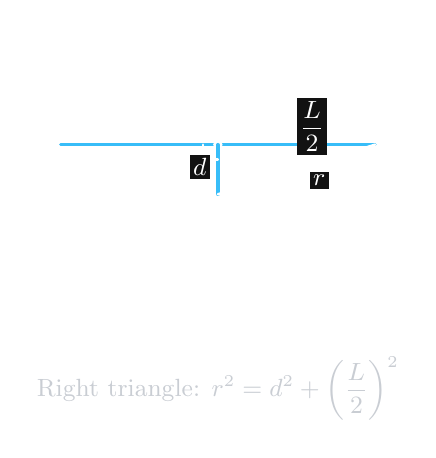
\begin{tikzpicture}[scale=1.05]
  \def\r{2.0}
  \coordinate (O) at (0,0);
  \coordinate (A) at ({-\r*0.95},0.6);
  \coordinate (B) at ({ \r*0.95},0.6);
  \coordinate (M) at ($(A)!0.5!(B)$);

  % circle
  \draw[base] (O) circle (\r);
  \node[dot] at (O) {};
  \node[lab] at ($(O)+(0,-0.28)$) {$O$};

  % chord + midpoint + perpendicular
  \draw[new] (A) -- (B);
  \node[dot] at (M) {};
  \node[lab] at ($(M)+(0,0.26)$) {$M$}; % moved up (fixes clash)
  \draw[new] (O) -- (M);

  % right angle mark at M
  \draw[base] ($(M)+(-0.18,0)$) -- ($(M)+(-0.18,-0.18)$) -- ($(M)+(0,-0.18)$);

  % radius to endpoint for triangle
  \draw[base] (O) -- (B);

  % labels (filled so lines don't cut through text)
  \node[lab, fill=pairbg, inner sep=1.2pt] at ($(O)!0.55!(M)+(-0.22,0)$) {$d$};
  \node[lab, fill=pairbg, inner sep=1.2pt] at ($(M)!0.60!(B)+(0,0.22)$) {$\dfrac{L}{2}$};
  \node[lab, fill=pairbg, inner sep=1.2pt] at ($(O)!0.55!(B)+(0.18,-0.16)$) {$r$};

  \node[labm] at (0,-2.35) {Right triangle: $r^2=d^2+\left(\dfrac{L}{2}\right)^2$};
\end{tikzpicture}
\end{StepDiagram}


\item \textbf{Equal chords are equidistant from the centre.}
\begin{StepDiagram}
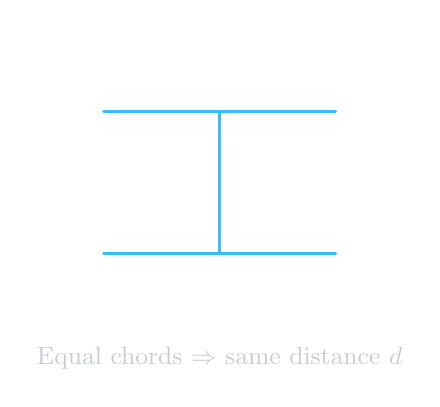
\begin{tikzpicture}[scale=0.95]
  \def\r{2.05}
  \coordinate (O) at (0,0);
  \coordinate (A1) at (-1.55, 0.95);
  \coordinate (B1) at ( 1.55, 0.95);
  \coordinate (A2) at (-1.55,-0.95);
  \coordinate (B2) at ( 1.55,-0.95);
  \coordinate (M1) at (0,0.95);
  \coordinate (M2) at (0,-0.95);

  \draw[base] (O) circle (\r);
  \node[dot,label={[lab]right:$O$}] at (O) {};

  \draw[new] (A1)--(B1);
  \draw[new] (A2)--(B2);

  \draw[new] (O)--(M1);
  \draw[new] (O)--(M2);

  \node[lab] at (-0.55,0.55) {$d$};
  \node[lab] at (-0.55,-0.55) {$d$};
  \node[labm] at (0,-2.35) {Equal chords $\Rightarrow$ same distance $d$};
\end{tikzpicture}
\end{StepDiagram}

\item \textbf{Perpendicular from centre bisects the chord.}
\begin{StepDiagram}
\begin{tikzpicture}[scale=0.95]
  \def\r{2.05}
  \coordinate (O) at (0,0);
  \coordinate (A) at (-1.70,0.70);
  \coordinate (B) at ( 1.70,0.70);
  \coordinate (M) at (0,0.70);

  \draw[base] (O) circle (\r);
  \node[dot,label={[lab]below:$O$}] at (O) {};

  \draw[new] (A)--(B);
  \node[dot,label={[lab]above:$M$}] at (M) {};
  \draw[new] (O)--(M);

  \draw[base] ($(M)+(-0.18,0)$) -- ($(M)+(-0.18,-0.18)$) -- ($(M)+(0,-0.18)$);

  \node[lab] at (-0.85,0.95) {$\dfrac{L}{2}$};
  \node[lab] at ( 0.85,0.95) {$\dfrac{L}{2}$};
  \node[labm] at (0,-2.35) {$OM\perp AB \Rightarrow AM=MB$};
\end{tikzpicture}
\end{StepDiagram}
\end{itemize}
\end{QuickBox}

% ============================================================
% Q1
\begin{QAPair}{Question 1}
\textcolor{gold}{\bfseries Question:} In the figure, $O$ is the centre of the circle and $\angle COF=150^\circ$.
Find $\angle OCF$ and $\angle CFD$.
\tcblower
\textcolor{green}{\bfseries Answer:}\par

\Step{1} Join $OC$ and $OF$. Since $OC=OF$ (radii), $\triangle OCF$ is isosceles.
\begin{StepDiagram}
\begin{tikzpicture}[scale=0.95]
  \def\r{2.1}
  \coordinate (O) at (0,0);
  \coordinate (C) at ({\r*cos(160)},{\r*sin(160)});
  \coordinate (F) at ({\r*cos(10)},{\r*sin(10)});
  \draw[base] (O) circle (\r);
  \node[dot,label={[lab]below:$O$}] at (O) {};
  \node[dot,label={[lab]left:$C$}] at (C) {};
  \node[dot,label={[lab]right:$F$}] at (F) {};
  \draw[new] (O)--(C);
  \draw[new] (O)--(F);
  \draw[base] (C)--(F);
  \pic[ang,"$150^\circ$",lab,angle radius=9mm,angle eccentricity=1.15] {angle=F--O--C};
\end{tikzpicture}
\end{StepDiagram}

\Step{2} Base angles are equal:
\[
\angle OCF=\angle OFC=\frac{180^\circ-150^\circ}{2}=15^\circ.
\]
\begin{StepDiagram}
\begin{tikzpicture}[scale=0.95]
  \def\r{2.1}
  \coordinate (O) at (0,0);
  \coordinate (C) at ({\r*cos(160)},{\r*sin(160)});
  \coordinate (F) at ({\r*cos(10)},{\r*sin(10)});
  \draw[base] (O) circle (\r);
  \node[dot,label={[lab]below:$O$}] at (O) {};
  \node[dot,label={[lab]left:$C$}] at (C) {};
  \node[dot,label={[lab]right:$F$}] at (F) {};
  \draw[new] (O)--(C);
  \draw[new] (O)--(F);
  \draw[base] (C)--(F);
  \pic[ang,"$15^\circ$",lab,angle radius=7mm,angle eccentricity=1.15] {angle=O--C--F};
  \pic[ang,"$15^\circ$",lab,angle radius=7mm,angle eccentricity=1.15] {angle=C--F--O};
\end{tikzpicture}
\end{StepDiagram}

\Step{3} The angle in the same segment (inscribed angle) subtending chord $CF$ is
\[
\frac12\angle COF=\frac{150^\circ}{2}=75^\circ.
\]
\begin{StepDiagram}
\begin{tikzpicture}[scale=0.95]
  \def\r{2.1}
  \coordinate (O) at (0,0);
  \coordinate (C) at ({\r*cos(160)},{\r*sin(160)});
  \coordinate (F) at ({\r*cos(10)},{\r*sin(10)});
  \coordinate (D) at ({\r*cos(70)},{\r*sin(70)});
  \draw[base] (O) circle (\r);
  \node[dot,label={[lab]below:$O$}] at (O) {};
  \node[dot,label={[lab]left:$C$}] at (C) {};
  \node[dot,label={[lab]right:$F$}] at (F) {};
  \node[dot,label={[lab]above:$D$}] at (D) {};
  \draw[base] (C)--(F);
  \draw[new] (D)--(C);
  \draw[new] (D)--(F);
  \pic[ang,"$75^\circ$",lab,angle radius=8mm,angle eccentricity=1.2] {angle=C--D--F};
\end{tikzpicture}
\end{StepDiagram}

\Step{4} By the tangent--chord theorem, the angle between chord $CF$ and tangent at $F$ equals the angle in the opposite segment.
Hence $\angle CFD=75^\circ$.
\begin{StepDiagram}
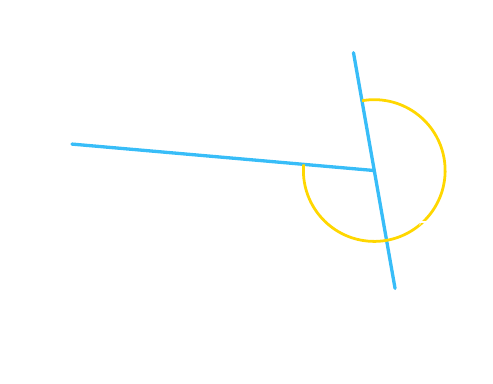
\begin{tikzpicture}[scale=0.95]
  \def\r{2.1}
  \coordinate (O) at (0,0);
  \coordinate (C) at ({\r*cos(160)},{\r*sin(160)});
  \coordinate (F) at ({\r*cos(10)},{\r*sin(10)});
  \coordinate (T1) at ($(F)+({-1.6*sin(10)},{1.6*cos(10)})$);
  \coordinate (T2) at ($(F)+({1.6*sin(10)},{-1.6*cos(10)})$);
  \coordinate (D) at ($(F)+({-1.4*sin(10)},{1.4*cos(10)})$);

  \draw[base] (O) circle (\r);
  \node[dot,label={[lab]below:$O$}] at (O) {};
  \node[dot,label={[lab]left:$C$}] at (C) {};
  \node[dot,label={[lab]right:$F$}] at (F) {};
  \node[dot,label={[lab]above left:$D$}] at (D) {};

  \draw[base] (O)--(F);
  \draw[new] (C)--(F);
  \draw[new] (T1)--(T2);

  \pic[ang,"$75^\circ$",lab,angle radius=9mm,angle eccentricity=1.2] {angle=C--F--D};
\end{tikzpicture}
\end{StepDiagram}

\[
\boxed{\angle OCF=15^\circ \qquad \angle CFD=75^\circ}
\]
\end{QAPair}

% ============================================================
% Q2
\begin{QAPair}{Question 2}
\textcolor{gold}{\bfseries Question:} Two circles of radius $3$ cm each are drawn with centres $P$ and $Q$.
$AB$ and $CD$ are chords such that $AB=CD=4$ cm.
Find the shortest distances of the chords from their respective centres. Are they equal?
\tcblower
\textcolor{green}{\bfseries Answer:}\par

\Step{1} Drop a perpendicular from the centre to each chord (it bisects the chord).
So $\dfrac{AB}{2}=\dfrac{CD}{2}=2$ cm.
\begin{StepDiagram}
\begin{tikzpicture}[scale=0.90]
  \def\r{2.1}
  \coordinate (P) at (0,0);
  \coordinate (A) at (-1.65,0.85);
  \coordinate (B) at ( 1.65,0.85);
  \coordinate (M) at (0,0.85);

  \draw[base] (P) circle (\r);
  \node[dot,label={[lab]below:$P$}] at (P) {};
  \draw[new] (A)--(B);
  \node[dot,label={[lab]above:$M$}] at (M) {};
  \draw[new] (P)--(M);
  \draw[base] ($(M)+(-0.18,0)$) -- ($(M)+(-0.18,-0.18)$) -- ($(M)+(0,-0.18)$);
  \node[lab] at (-0.85,1.12) {$2$};
  \node[lab] at ( 0.85,1.12) {$2$};
\end{tikzpicture}
\end{StepDiagram}

\Step{2} Use $r^2=d^2+\left(\dfrac{L}{2}\right)^2$:
\[
3^2=d^2+2^2 \;\Rightarrow\; d^2=5 \;\Rightarrow\; d=\sqrt5\text{ cm}.
\]
\EqDiagram{$3^2=d^2+2^2 \;\Rightarrow\; d=\sqrt{5}\text{ cm}$}

\Step{3} Since both circles have the same radius and both chords have the same length, the shortest distances must be equal.
\begin{StepDiagram}
\begin{tikzpicture}[scale=0.90]
  \def\r{1.45}
  \coordinate (P) at (-2.2,0);
  \coordinate (Q) at ( 2.2,0);
  \draw[base] (P) circle (\r);
  \draw[base] (Q) circle (\r);
  \node[dot,label={[lab]below:$P$}] at (P) {};
  \node[dot,label={[lab]below:$Q$}] at (Q) {};

  \draw[new] ($(P)+(-1.05,0.55)$) -- ($(P)+(1.05,0.55)$);
  \draw[new] ($(Q)+(-1.05,-0.55)$) -- ($(Q)+(1.05,-0.55)$);

  \node[labm] at (0,-1.9) {$r$ same and chord length same $\Rightarrow$ distance from centre same};
\end{tikzpicture}
\end{StepDiagram}

\[
\boxed{\text{Shortest distance}=\sqrt{5}\text{ cm for each chord, so they are equal.}}
\]
\end{QAPair}

% ============================================================
% Q3
\begin{QAPair}{Question 3}
\textcolor{gold}{\bfseries Question:} Find the distance between two chords $PQ$ and $RS$ of a circle if
$PQ=6$ cm, $RS=8$ cm and radius $=5$ cm.
\tcblower
\textcolor{green}{\bfseries Answer:}\par

\Step{1} Distance from centre to chord $PQ$:
\[
d_{PQ}=\sqrt{5^2-\left(\frac{6}{2}\right)^2}=\sqrt{25-9}=4.
\]
\begin{StepDiagram}
\begin{tikzpicture}[scale=0.90]
  \def\r{2.2}
  \coordinate (O) at (0,0);
  \coordinate (P) at (-1.25,1.15);
  \coordinate (Q) at ( 1.25,1.15);
  \coordinate (M) at (0,1.15);

  \draw[base] (O) circle (\r);
  \node[dot,label={[lab]below:$O$}] at (O) {};
  \draw[new] (P)--(Q);
  \node[dot,label={[lab]above:$T$}] at (M) {};
  \draw[new] (O)--(M);
  \draw[base] ($(M)+(-0.18,0)$) -- ($(M)+(-0.18,-0.18)$) -- ($(M)+(0,-0.18)$);
  \node[lab] at ($(O)!0.5!(M)+(-0.35,0)$) {$4$};
  \node[lab] at ($(P)!0.5!(M)+(0,0.25)$) {$3$};
\end{tikzpicture}
\end{StepDiagram}

\Step{2} Distance from centre to chord $RS$:
\[
d_{RS}=\sqrt{5^2-\left(\frac{8}{2}\right)^2}=\sqrt{25-16}=3.
\]
\begin{StepDiagram}
\begin{tikzpicture}[scale=0.90]
  \def\r{2.2}
  \coordinate (O) at (0,0);
  \coordinate (R) at (-1.65,-1.15);
  \coordinate (S) at ( 1.65,-1.15);
  \coordinate (N) at (0,-1.15);

  \draw[base] (O) circle (\r);
  \node[dot,label={[lab]above:$O$}] at (O) {};
  \draw[new] (R)--(S);
  \node[dot,label={[lab]below:$U$}] at (N) {};
  \draw[new] (O)--(N);
  \draw[base] ($(N)+(-0.18,0)$) -- ($(N)+(-0.18,0.18)$) -- ($(N)+(0,0.18)$);
  \node[lab] at ($(O)!0.5!(N)+(-0.35,0)$) {$3$};
  \node[lab] at ($(R)!0.5!(N)+(0,-0.25)$) {$4$};
\end{tikzpicture}
\end{StepDiagram}

\Step{3} From the figure, chords are on \emph{opposite sides} of the centre, so distance between them is
\[
d_{PQ}+d_{RS}=4+3=7.
\]
\EqDiagram{Opposite sides: distance $=d_{PQ}+d_{RS}=4+3=7$}

\[
\boxed{7\text{ cm}}
\]
\end{QAPair}

% ============================================================
% Q4(i)
\begin{QAPair}{Question 4 (i)}
\textcolor{gold}{\bfseries Question:} In the circle, $O$ is the centre. Find the unknowns $y$ and $a$ (all lengths in cm).
\tcblower
\textcolor{green}{\bfseries Answer:}\par

\Step{1} $r=15$, chord $=18 \Rightarrow \dfrac{18}{2}=9$. Drop $OM\perp$ chord.
\begin{StepDiagram}
\begin{tikzpicture}[scale=0.90]
  \def\r{2.4}
  \coordinate (O) at (0,0);
  \coordinate (A) at ({\r*cos(130)},{\r*sin(130)});
  \coordinate (B) at ({\r*cos(50)},{\r*sin(50)});
  \coordinate (M) at ($(A)!0.5!(B)$);

  \draw[base] (O) circle (\r);
  \node[dot,label={[lab]right:$O$}] at (O) {};
  \draw[new] (A)--(B);
  \node[dot,label={[lab]above:$M$}] at (M) {};
  \draw[new] (O)--(M);
  \draw[base] ($(M)+(-0.18,0)$) -- ($(M)+(-0.18,-0.18)$) -- ($(M)+(0,-0.18)$);
  \draw[base] (O)--(A);
  \node[lab] at ($(A)!0.5!(M)+(-0.1,0.35)$) {$9$};
  \node[lab] at ($(O)!0.55!(A)+(-0.2,0.1)$) {$15$};
\end{tikzpicture}
\end{StepDiagram}

\Step{2} Use the right triangle $OAM$:
\[
OM=\sqrt{15^2-9^2}=\sqrt{225-81}=\sqrt{144}=12.
\]
\begin{StepDiagram}
\begin{tikzpicture}[scale=0.90]
  \def\r{2.4}
  \coordinate (O) at (0,0);
  \coordinate (A) at ({\r*cos(130)},{\r*sin(130)});
  \coordinate (B) at ({\r*cos(50)},{\r*sin(50)});
  \coordinate (M) at ($(A)!0.5!(B)$);

  \draw[base] (O) circle (\r);
  \node[dot,label={[lab]right:$O$}] at (O) {};
  \draw[new] (A)--(B);
  \node[dot,label={[lab]above:$M$}] at (M) {};
  \draw[new] (O)--(M);
  \draw[base] (O)--(A);
  \draw[base] ($(M)+(-0.18,0)$) -- ($(M)+(-0.18,-0.18)$) -- ($(M)+(0,-0.18)$);
  \node[lab] at ($(O)!0.5!(M)+(-0.35,0)$) {$12$};
  \node[lab] at ($(A)!0.5!(M)+(-0.1,0.35)$) {$9$};
\end{tikzpicture}
\end{StepDiagram}

\Step{3} For angle $y$ in right $\triangle OAM$:
\[
\cos y=\frac{AM}{OA}=\frac{9}{15}=\frac35
\Rightarrow y=\cos^{-1}\!\left(\frac35\right)\approx 53.13^\circ.
\]
\EqDiagram{$\cos y=\dfrac{9}{15}=\dfrac35 \Rightarrow y\approx 53.13^\circ$}

\Step{4} For the lower chord $24$:
\[
\frac{24}{2}=12,\qquad
a=\sqrt{15^2-12^2}=\sqrt{225-144}=9.
\]
\begin{StepDiagram}
\begin{tikzpicture}[scale=0.90]
  \def\r{2.4}
  \coordinate (O) at (0,0);
  \coordinate (R) at ({\r*cos(210)},{\r*sin(210)});
  \coordinate (S) at ({\r*cos(330)},{\r*sin(330)});
  \coordinate (N) at ($(R)!0.5!(S)$);

  \draw[base] (O) circle (\r);
  \node[dot,label={[lab]right:$O$}] at (O) {};
  \draw[new] (R)--(S);
  \node[dot,label={[lab]below:$N$}] at (N) {};
  \draw[new] (O)--(N);
  \draw[base] ($(N)+(-0.18,0)$) -- ($(N)+(-0.18,0.18)$) -- ($(N)+(0,0.18)$);
  \node[lab] at ($(O)!0.5!(N)+(-0.45,0)$) {$a=9$};
  \node[lab] at ($(R)!0.5!(N)+(0,-0.25)$) {$12$};
\end{tikzpicture}
\end{StepDiagram}

\[
\boxed{y\approx 53.13^\circ \qquad a=9\text{ cm}}
\]
\end{QAPair}

% ============================================================
% Q4(ii)
\begin{QAPair}{Question 4 (ii)}
\textcolor{gold}{\bfseries Question:} In the circle, $O$ is the centre. Find the unknowns $x$, $y$, and $a$ (all lengths in cm).
\tcblower
\textcolor{green}{\bfseries Answer:}\par

\Step{1} The lower chord has length $12 \Rightarrow \dfrac{12}{2}=6$, and its distance from $O$ is $6$.
\begin{StepDiagram}
\begin{tikzpicture}[scale=0.90]
  \def\r{2.35}
  \coordinate (O) at (0,0);
  \coordinate (L1) at (-1.7,-1.2);
  \coordinate (L2) at (1.7,-1.2);
  \coordinate (M) at (0,-1.2);

  \draw[base] (O) circle (\r);
  \node[dot,label={[lab]right:$O$}] at (O) {};
  \draw[new] (L1)--(L2);
  \node[dot,label={[lab]below:$M$}] at (M) {};
  \draw[new] (O)--(M);
  \draw[base] ($(M)+(-0.18,0)$) -- ($(M)+(-0.18,0.18)$) -- ($(M)+(0,0.18)$);
  \node[lab] at ($(L1)!0.5!(M)+(0,-0.25)$) {$6$};
  \node[lab] at ($(O)!0.5!(M)+(-0.35,0)$) {$6$};
\end{tikzpicture}
\end{StepDiagram}

\Step{2} Radius is the hypotenuse:
\[
y=\sqrt{6^2+6^2}=6\sqrt2.
\]
\EqDiagram{$y=\sqrt{6^2+6^2}=6\sqrt2$}

\Step{3} For the top chord (also $12$ cm), the perpendicular bisects it, so $x=6$.
\begin{StepDiagram}
\begin{tikzpicture}[scale=0.90]
  \def\r{2.35}
  \coordinate (O) at (0,0);
  \coordinate (A) at (-1.7,1.2);
  \coordinate (B) at (1.7,1.2);
  \coordinate (M) at (0,1.2);

  \draw[base] (O) circle (\r);
  \node[dot,label={[lab]right:$O$}] at (O) {};
  \draw[new] (A)--(B);
  \node[dot,label={[lab]above:$M$}] at (M) {};
  \draw[new] (O)--(M);
  \draw[base] ($(M)+(-0.18,0)$) -- ($(M)+(-0.18,-0.18)$) -- ($(M)+(0,-0.18)$);
  \node[lab] at ($(A)!0.5!(M)+(0,0.25)$) {$x=6$};
\end{tikzpicture}
\end{StepDiagram}

\Step{4} Equal chords are equidistant from the centre, hence $a=6$.
\begin{StepDiagram}
\begin{tikzpicture}[scale=0.90]
  \def\r{2.35}
  \coordinate (O) at (0,0);
  \coordinate (M1) at (0,1.2);
  \coordinate (M2) at (0,-1.2);
  \draw[base] (O) circle (\r);
  \node[dot,label={[lab]right:$O$}] at (O) {};
  \draw[new] (O)--(M1);
  \draw[new] (O)--(M2);
  \node[lab] at ($(O)!0.5!(M1)+(-0.35,0)$) {$a$};
  \node[lab] at ($(O)!0.5!(M2)+(-0.35,0)$) {$a$};
  \node[labm] at (0,-2.55) {Equal chords $\Rightarrow$ equal distances};
\end{tikzpicture}
\end{StepDiagram}

\[
\boxed{x=6\text{ cm}\qquad y=6\sqrt{2}\text{ cm}\qquad a=6\text{ cm}}
\]
\end{QAPair}

% ============================================================
% Q5
\begin{QAPair}{Question 5}
\textcolor{gold}{\bfseries Question:} Two parallel chords of lengths $24$ cm and $12$ cm are drawn on opposite sides of a circle of radius $13$ cm. Find the distance between the chords.
\tcblower
\textcolor{green}{\bfseries Answer:}\par

\Step{1} Distance to the $24$ cm chord:
\[
d_{24}=\sqrt{13^2-\left(\frac{24}{2}\right)^2}=\sqrt{169-144}=5.
\]
\begin{StepDiagram}
\begin{tikzpicture}[scale=0.90]
  \def\r{2.35}
  \coordinate (O) at (0,0);
  \coordinate (T1) at (-1.95,1.05);
  \coordinate (T2) at ( 1.95,1.05);
  \coordinate (M1) at (0,1.05);

  \draw[base] (O) circle (\r);
  \node[dot,label={[lab]right:$O$}] at (O) {};
  \draw[new] (T1)--(T2);
  \draw[new] (O)--(M1);
  \node[lab] at ($(O)!0.5!(M1)+(-0.35,0)$) {$5$};
  \node[lab] at (-0.95,1.30) {$12$};
  \node[lab] at ( 0.95,1.30) {$12$};
\end{tikzpicture}
\end{StepDiagram}

\Step{2} Distance to the $12$ cm chord:
\[
d_{12}=\sqrt{13^2-\left(\frac{12}{2}\right)^2}=\sqrt{169-36}=\sqrt{133}.
\]
\begin{StepDiagram}
\begin{tikzpicture}[scale=0.90]
  \def\r{2.35}
  \coordinate (O) at (0,0);
  \coordinate (B1) at (-1.25,-1.15);
  \coordinate (B2) at ( 1.25,-1.15);
  \coordinate (M2) at (0,-1.15);

  \draw[base] (O) circle (\r);
  \node[dot,label={[lab]right:$O$}] at (O) {};
  \draw[new] (B1)--(B2);
  \draw[new] (O)--(M2);
  \node[lab] at ($(O)!0.5!(M2)+(-0.55,0)$) {$\sqrt{133}$};
  \node[lab] at (-0.60,-1.40) {$6$};
  \node[lab] at ( 0.60,-1.40) {$6$};
\end{tikzpicture}
\end{StepDiagram}

\Step{3} Opposite sides $\Rightarrow$ distance between chords $=d_{24}+d_{12}=5+\sqrt{133}$.
\EqDiagram{Distance $=5+\sqrt{133}\text{ cm}$}

\[
\boxed{5+\sqrt{133}\text{ cm}}
\]
\end{QAPair}

% ============================================================
% Q6
\begin{QAPair}{Question 6}
\textcolor{gold}{\bfseries Question:} $AB$ is a chord of a bigger circle of radius $10$ cm centred at $O$.
If $AB=16$ cm, find the radius of the smaller circle passing through the midpoint of $AB$.
Also find the difference of radii.
\tcblower
\textcolor{green}{\bfseries Answer:}\par

\Step{1} $\dfrac{AB}{2}=8$. Drop $OM\perp AB$:
\[
OM=\sqrt{10^2-8^2}=\sqrt{100-64}=6.
\]
\begin{StepDiagram}
\begin{tikzpicture}[scale=0.90]
  \def\r{2.35}
  \coordinate (O) at (0,0);
  \coordinate (A) at (-1.85,1.00);
  \coordinate (B) at ( 1.85,1.00);
  \coordinate (M) at (0,1.00);

  \draw[base] (O) circle (\r);
  \node[dot,label={[lab]below:$O$}] at (O) {};
  \draw[new] (A)--(B);
  \node[dot,label={[lab]above:$M$}] at (M) {};
  \draw[new] (O)--(M);
  \draw[base] ($(M)+(-0.18,0)$) -- ($(M)+(-0.18,-0.18)$) -- ($(M)+(0,-0.18)$);
  \node[lab] at ($(A)!0.5!(M)+(0,0.25)$) {$8$};
  \node[lab] at ($(O)!0.5!(M)+(-0.35,0)$) {$6$};
\end{tikzpicture}
\end{StepDiagram}

\Step{2} The smaller circle is concentric (same centre $O$) and passes through $M$,
so its radius is $r_{\text{small}}=OM=6$.
\begin{StepDiagram}

\begin{tikzpicture}[scale=0.90]
  \def\R{2.35}
  \def\rS{1.41} % (6/10)*R
  \coordinate (O) at (0,0);
  \coordinate (M) at (0,1.00);

  \draw[base] (O) circle (\R);
  \draw[new]  (O) circle (\rS);
  \node[dot,label={[lab]below:$O$}] at (O) {};
  \node[dot,label={[lab]right:$M$}] at (M) {};
  \draw[new] (O)--(M);
  \node[lab] at ($(O)!0.5!(M)+(0.35,0)$) {$6$};
\end{tikzpicture}
\end{StepDiagram}

\Step{3} Difference of radii:
\[
10-6=4.
\]
\EqDiagram{Difference $=10-6=4\text{ cm}$}

\[
\boxed{r_{\text{small}}=6\text{ cm}\qquad \text{difference}=4\text{ cm}}
\]
\end{QAPair}

% ============================================================
% Q7
\begin{QAPair}{Question 7}
\textcolor{gold}{\bfseries Question:} Two parallel chords of lengths $18$ cm and $80$ cm are drawn on the same side of a circle of radius $41$ cm. Find the distance between the chords.
\tcblower
\textcolor{green}{\bfseries Answer:}\par

\Step{1} For chord $80$:
\[
d_{80}=\sqrt{41^2-\left(\frac{80}{2}\right)^2}=\sqrt{1681-1600}=9.
\]
\begin{StepDiagram}
\begin{tikzpicture}[scale=0.90]
  \def\r{2.35}
  \coordinate (O) at (0,0);
  \coordinate (C1) at (-2.00,0.95);
  \coordinate (C2) at ( 2.00,0.95);
  \coordinate (M1) at (0,0.95);

  \draw[base] (O) circle (\r);
  \node[dot,label={[lab]below:$O$}] at (O) {};
  \draw[new] (C1)--(C2);
  \draw[new] (O)--(M1);
  \node[lab] at ($(O)!0.5!(M1)+(-0.35,0)$) {$9$};
  \node[labm] at (0,-2.55) {Longer chord is nearer to centre};
\end{tikzpicture}
\end{StepDiagram}

\Step{2} For chord $18$:
\[
d_{18}=\sqrt{41^2-\left(\frac{18}{2}\right)^2}=\sqrt{1681-81}=40.
\]
\begin{StepDiagram}
\begin{tikzpicture}[scale=0.90]
  \def\r{2.35}
  \coordinate (O) at (0,0);
  \coordinate (D1) at (-1.20,1.55);
  \coordinate (D2) at ( 1.20,1.55);
  \coordinate (M2) at (0,1.55);

  \draw[base] (O) circle (\r);
  \node[dot,label={[lab]below:$O$}] at (O) {};
  \draw[new] (D1)--(D2);
  \draw[new] (O)--(M2);
  \node[lab] at ($(O)!0.5!(M2)+(-0.45,0)$) {$40$};
\end{tikzpicture}
\end{StepDiagram}

\Step{3} Same side $\Rightarrow$ distance between chords $=40-9=31$ cm.
\EqDiagram{Distance $=40-9=31\text{ cm}$}

\[
\boxed{31\text{ cm}}
\]
\end{QAPair}

% ============================================================
% Q8
\begin{QAPair}{Question 8}
\textcolor{gold}{\bfseries Question:} Two parallel chords $AB$ and $CD$ are $4$ cm apart and lie on opposite sides of the centre.
If $AB=2$ cm and $CD=6$ cm, find the radius of the circle.
\tcblower
\textcolor{green}{\bfseries Answer:}\par

\Step{1} Half-chords:
\[
\frac{AB}{2}=1,\qquad \frac{CD}{2}=3.
\]
\begin{StepDiagram}
\begin{tikzpicture}[scale=0.90]
  \def\r{2.35}
  \coordinate (O) at (0,0);
  \coordinate (A) at (-0.70,1.40);
  \coordinate (B) at ( 0.70,1.40);
  \coordinate (C) at (-1.50,-1.20);
  \coordinate (D) at ( 1.50,-1.20);
  \coordinate (M1) at (0,1.40);
  \coordinate (M2) at (0,-1.20);

  \draw[base] (O) circle (\r);
  \node[dot,label={[lab]right:$O$}] at (O) {};
  \draw[new] (A)--(B);
  \draw[new] (C)--(D);
  \node[lab] at (-0.05,1.65) {$1$};
  \node[lab] at ( 0.05,-1.45) {$3$};
\end{tikzpicture}
\end{StepDiagram}

\Step{2} Let distances from centre be $d_1$ (to $AB$) and $d_2$ (to $CD$).
Opposite sides and $4$ cm apart $\Rightarrow d_1+d_2=4$.
\EqDiagram{Opposite sides: $d_1+d_2=4$}

\Step{3} Use right-triangle relation for each chord:
\[
r^2=d_1^2+1^2,\qquad r^2=d_2^2+3^2.
\]
\EqDiagram{$r^2=d_1^2+1,\quad r^2=d_2^2+9$}

\Step{4} Subtract:
\[
d_1^2+1=d_2^2+9 \Rightarrow d_1^2-d_2^2=8
\Rightarrow (d_1-d_2)(d_1+d_2)=8.
\]
\EqDiagram{$(d_1-d_2)(d_1+d_2)=8$}

\Step{5} Since $d_1+d_2=4$,
\[
(d_1-d_2)\cdot 4=8 \Rightarrow d_1-d_2=2
\Rightarrow d_1=3,\ d_2=1.
\]
\EqDiagram{$d_1=3,\ d_2=1$}

\Step{6} Find $r$:
\[
r^2=d_1^2+1=3^2+1=10 \Rightarrow r=\sqrt{10}.
\]
\EqDiagram{$r=\sqrt{10}\text{ cm}$}

\[
\boxed{r=\sqrt{10}\text{ cm}}
\]
\end{QAPair}

% ============================================================
% Q9
\begin{QAPair}{Question 9}
\textcolor{gold}{\bfseries Question:} $PQ$ and $RS$ are two parallel chords lying on the same side of the centre and are $2$ cm apart.
If $PQ=8$ cm and $RS=10$ cm, find the radius of the circle.
\tcblower
\textcolor{green}{\bfseries Answer:}\par

\Step{1} Half-chords:
\[
\frac{PQ}{2}=4,\qquad \frac{RS}{2}=5.
\]
\begin{StepDiagram}
\begin{tikzpicture}[scale=0.90]
  \def\r{2.35}
  \coordinate (O) at (0,0);
  \coordinate (P) at (-1.20,1.55);
  \coordinate (Q) at ( 1.20,1.55);
  \coordinate (R) at (-1.70,1.05);
  \coordinate (S) at ( 1.70,1.05);
  \draw[base] (O) circle (\r);
  \node[dot,label={[lab]below:$O$}] at (O) {};
  \draw[new] (P)--(Q);
  \draw[new] (R)--(S);
  \node[lab] at (0,1.80) {$4$};
  \node[lab] at (0,1.30) {$5$};
  \draw[help,<->] (2.05,1.55) -- (2.05,1.05);
  \node[lab] at (2.30,1.30) {$2$};
\end{tikzpicture}
\end{StepDiagram}

\Step{2} Let distances be $d_{PQ}$ and $d_{RS}$. Same side and $2$ cm apart:
\[
d_{PQ}-d_{RS}=2
\quad\text{(shorter chord is farther from centre).}
\]
\EqDiagram{Same side: $d_{PQ}-d_{RS}=2$}

\Step{3} Use the right-triangle relation:
\[
r^2=d_{PQ}^2+4^2,\qquad r^2=d_{RS}^2+5^2.
\]
\EqDiagram{$r^2=d_{PQ}^2+16,\quad r^2=d_{RS}^2+25$}

\Step{4} Subtract:
\[
d_{PQ}^2+16=d_{RS}^2+25
\Rightarrow d_{PQ}^2-d_{RS}^2=9
\Rightarrow (d_{PQ}-d_{RS})(d_{PQ}+d_{RS})=9.
\]
\EqDiagram{$(d_{PQ}-d_{RS})(d_{PQ}+d_{RS})=9$}

\Step{5} Since $d_{PQ}-d_{RS}=2$:
\[
2(d_{PQ}+d_{RS})=9 \Rightarrow d_{PQ}+d_{RS}=4.5.
\]
\EqDiagram{$d_{PQ}+d_{RS}=4.5$}

\Step{6} Solve:
\[
d_{PQ}=\frac{4.5+2}{2}=3.25,\qquad
d_{RS}=\frac{4.5-2}{2}=1.25.
\]
\EqDiagram{$d_{PQ}=3.25,\ d_{RS}=1.25$}

\Step{7} Find $r$:
\[
r^2=d_{RS}^2+25=1.25^2+25=26.5625=\frac{425}{16}
\Rightarrow r=\frac{\sqrt{425}}{4}=\frac{5\sqrt{17}}{4}.
\]
\EqDiagram{$r=\dfrac{5\sqrt{17}}{4}\text{ cm}$}

\[
\boxed{r=\frac{5\sqrt{17}}{4}\text{ cm}}
\]
\end{QAPair}

\end{document}
